% \begin{figure}%[!b]
% \begin{subfigure}{0.5\textwidth}
% 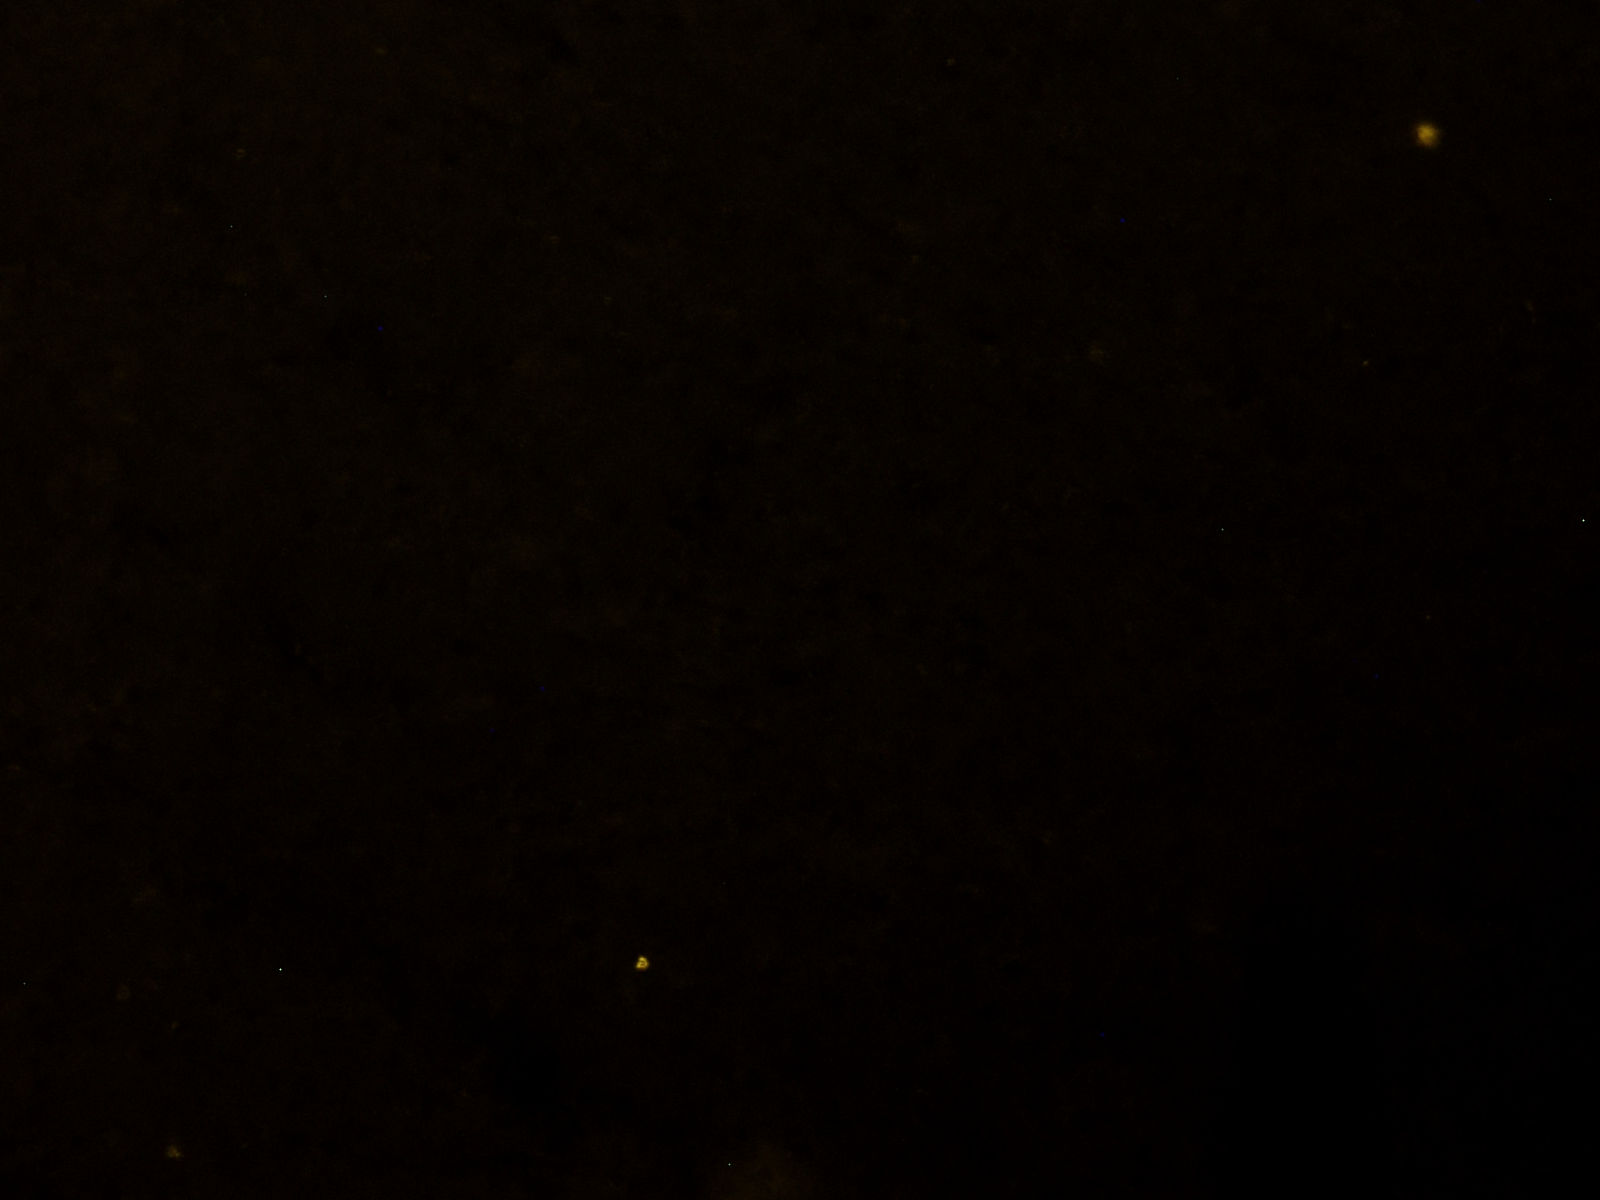
\includegraphics[width=\linewidth]{figures/120_dataset/i_empty.png}
% \subcaption{}
% \end{subfigure}%
% \begin{subfigure}{0.5\textwidth}
% 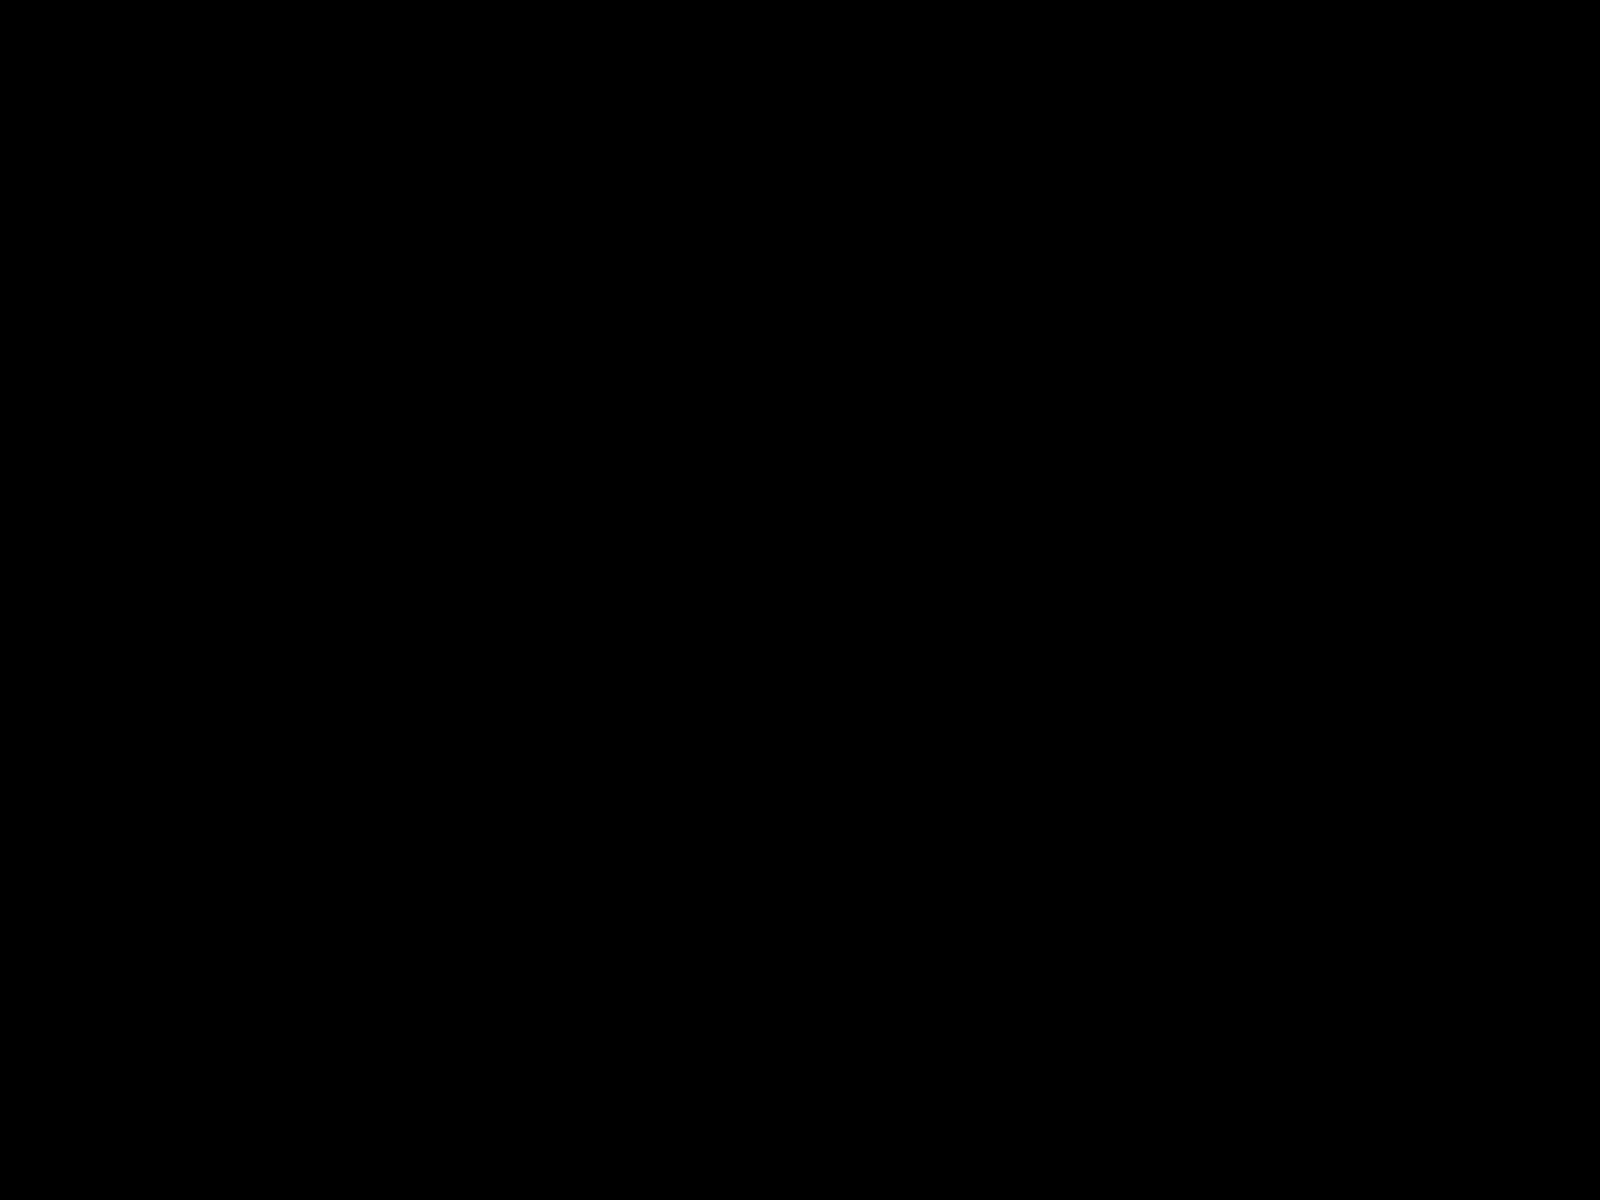
\includegraphics[width=\linewidth]{figures/120_dataset/m_empty.png}
% \subcaption{}
% \label{fig:dataset:empty}
% \end{subfigure}

% \centering
% \begin{subfigure}{0.5\textwidth}
% 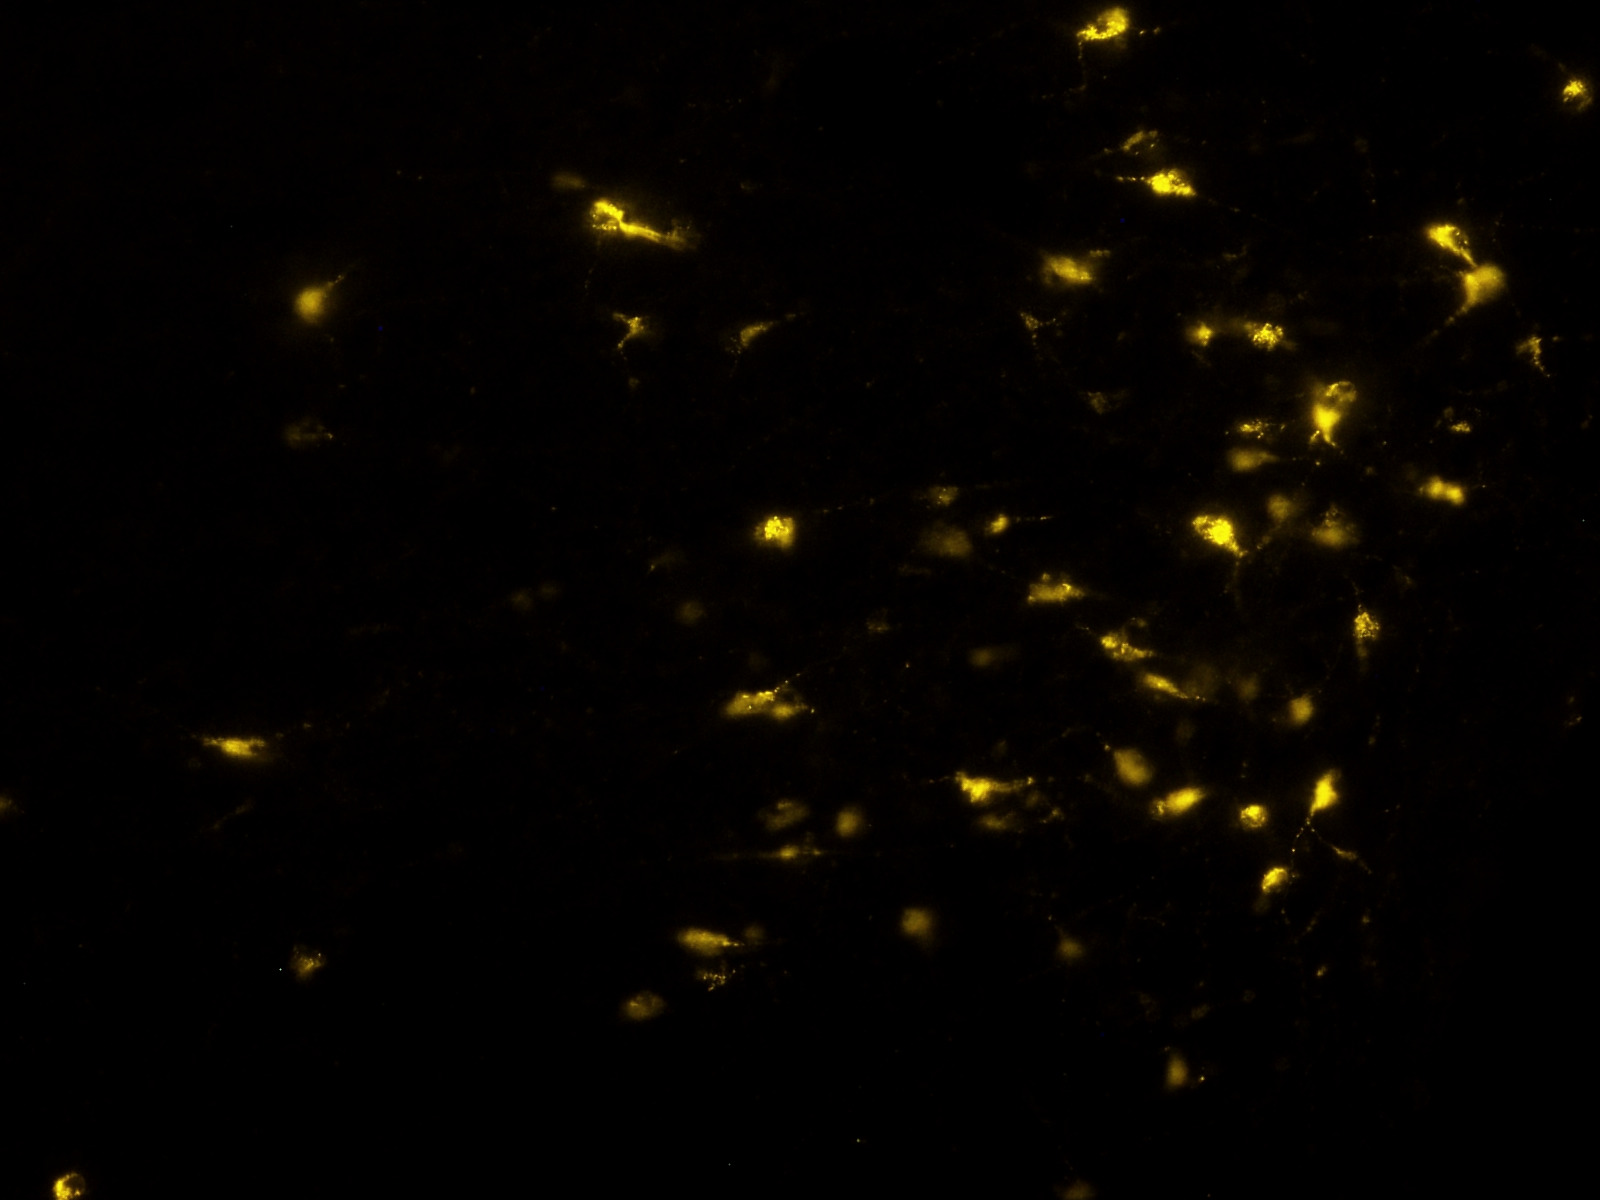
\includegraphics[width=\linewidth]{figures/120_dataset/i_168.jpeg}
% \subcaption{}
% \end{subfigure}%
% \begin{subfigure}{0.5\textwidth}
% 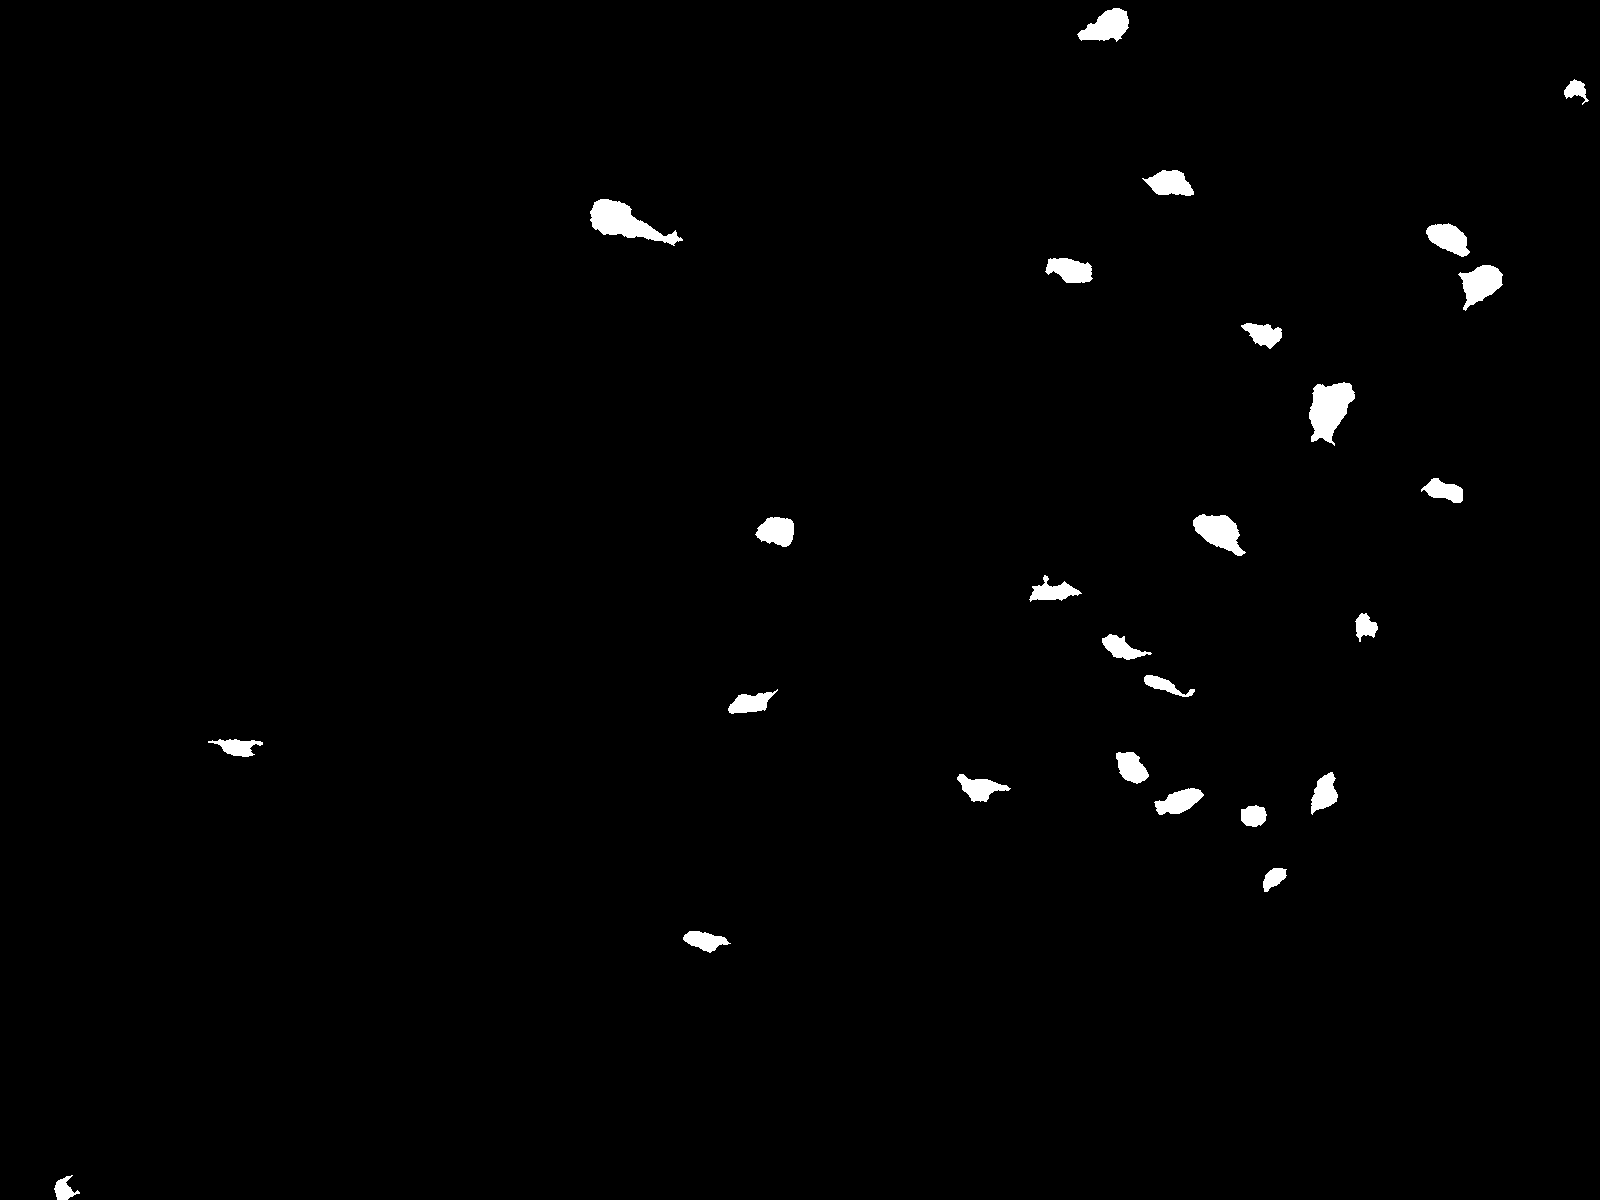
\includegraphics[width=\linewidth]{figures/120_dataset/m_168.png}
% \subcaption{}
% \label{fig:dataset:dark}
% \end{subfigure}

% \centering
% \begin{subfigure}{0.5\textwidth}
% 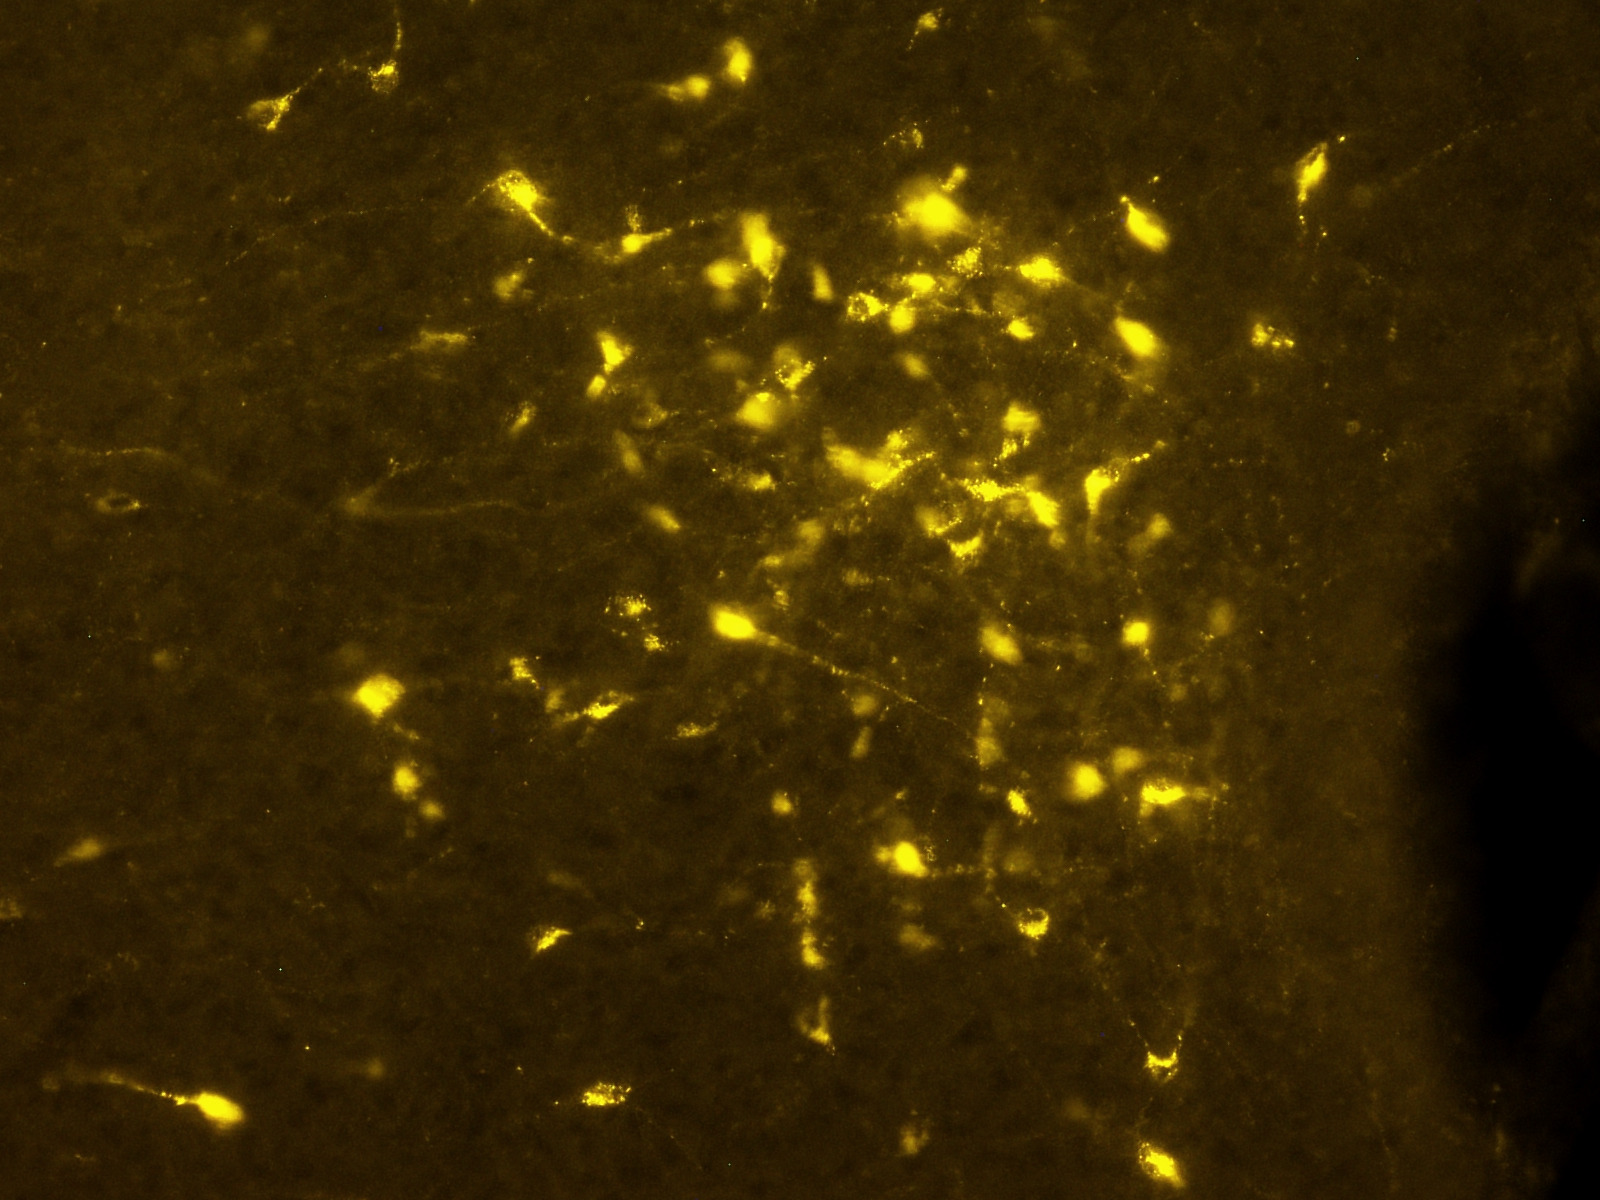
\includegraphics[width=\linewidth]{figures/120_dataset/i_257.jpeg}
% \subcaption{}
% \end{subfigure}%
% \begin{subfigure}{0.5\textwidth}
% 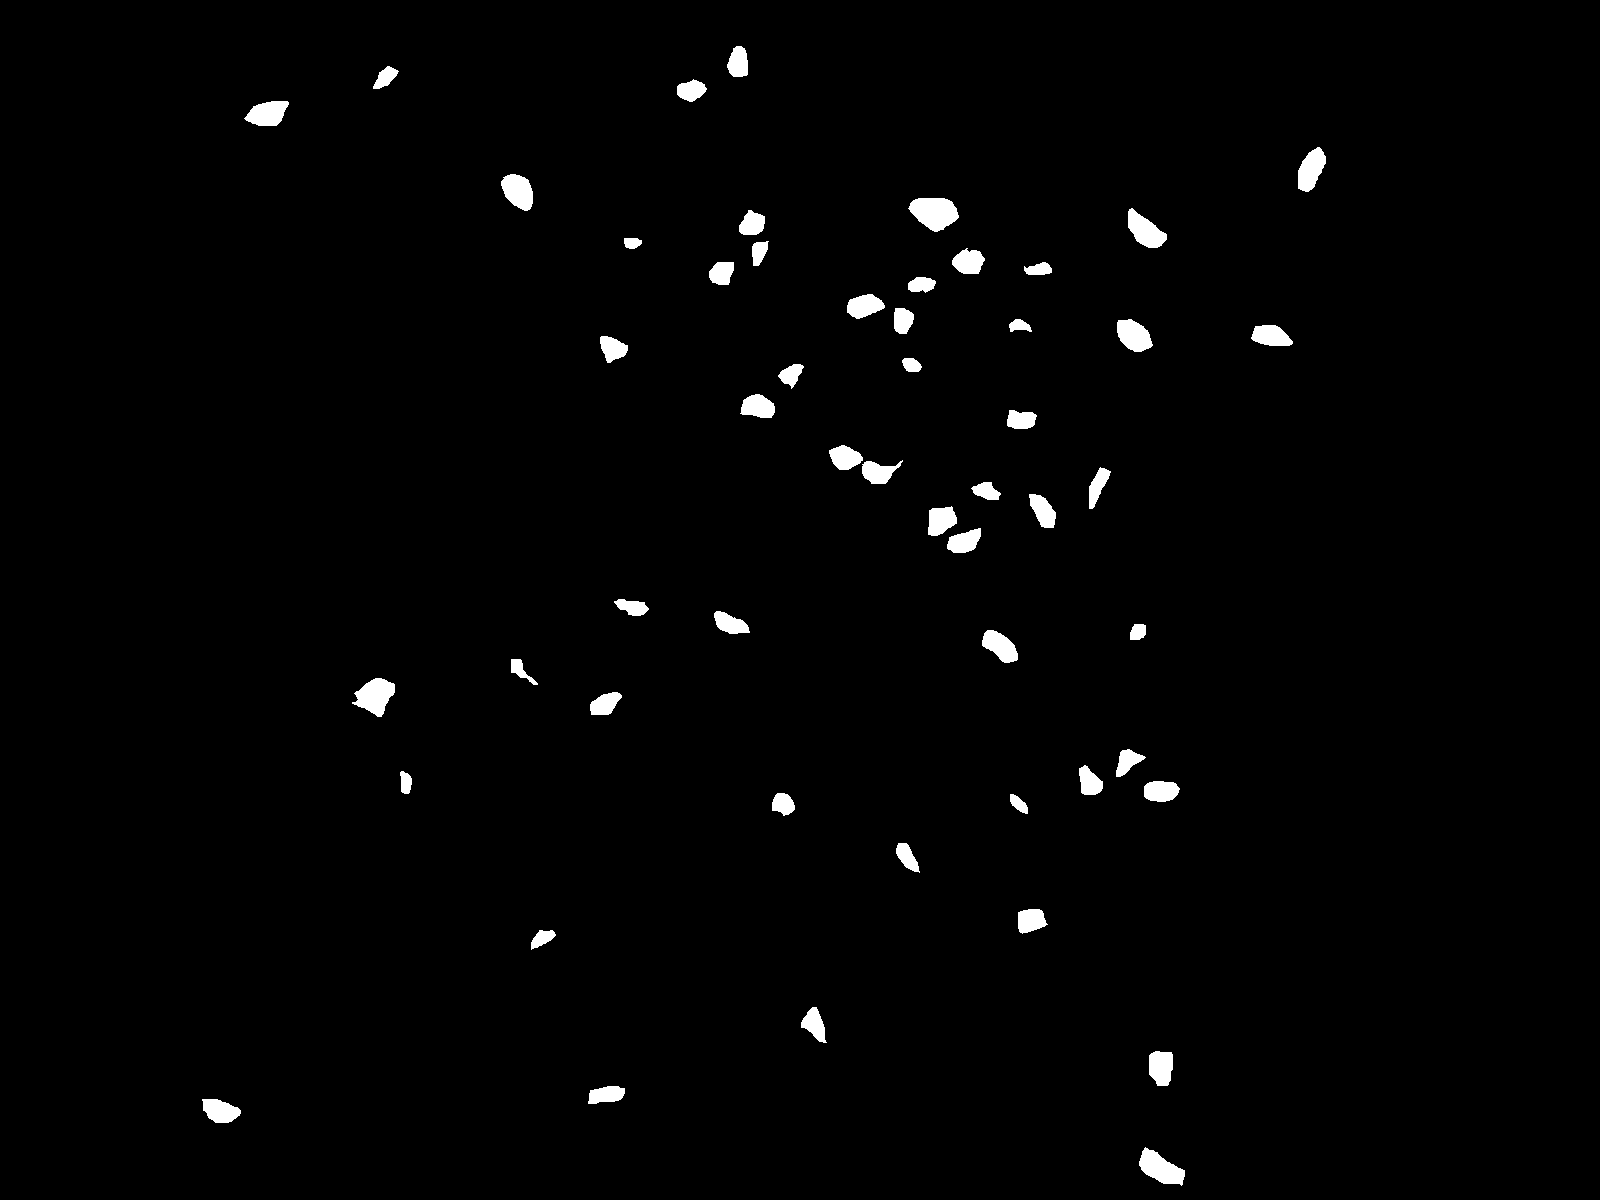
\includegraphics[width=\linewidth]{figures/120_dataset/m_257.png}
% \subcaption{}
% \label{fig:dataset:bright}
% \end{subfigure}
% \vspace{-0.2cm}
% \caption{
% \textbf{Sample data}. 
% Original images (left) and corresponding ground-truth masks (right).
% % The original images (left) present neuronal cells of different shape, size and saturation over a background of variable brightness and color.
% % The corresponding ground-truth masks used for training (right) depicts cells as white pixels over a black background.
% } \label{fig:dataset}
% \end{figure}%
% \begin{figure}%[ht]\ContinuedFloat
% \centering
% \begin{subfigure}{0.5\textwidth}
% 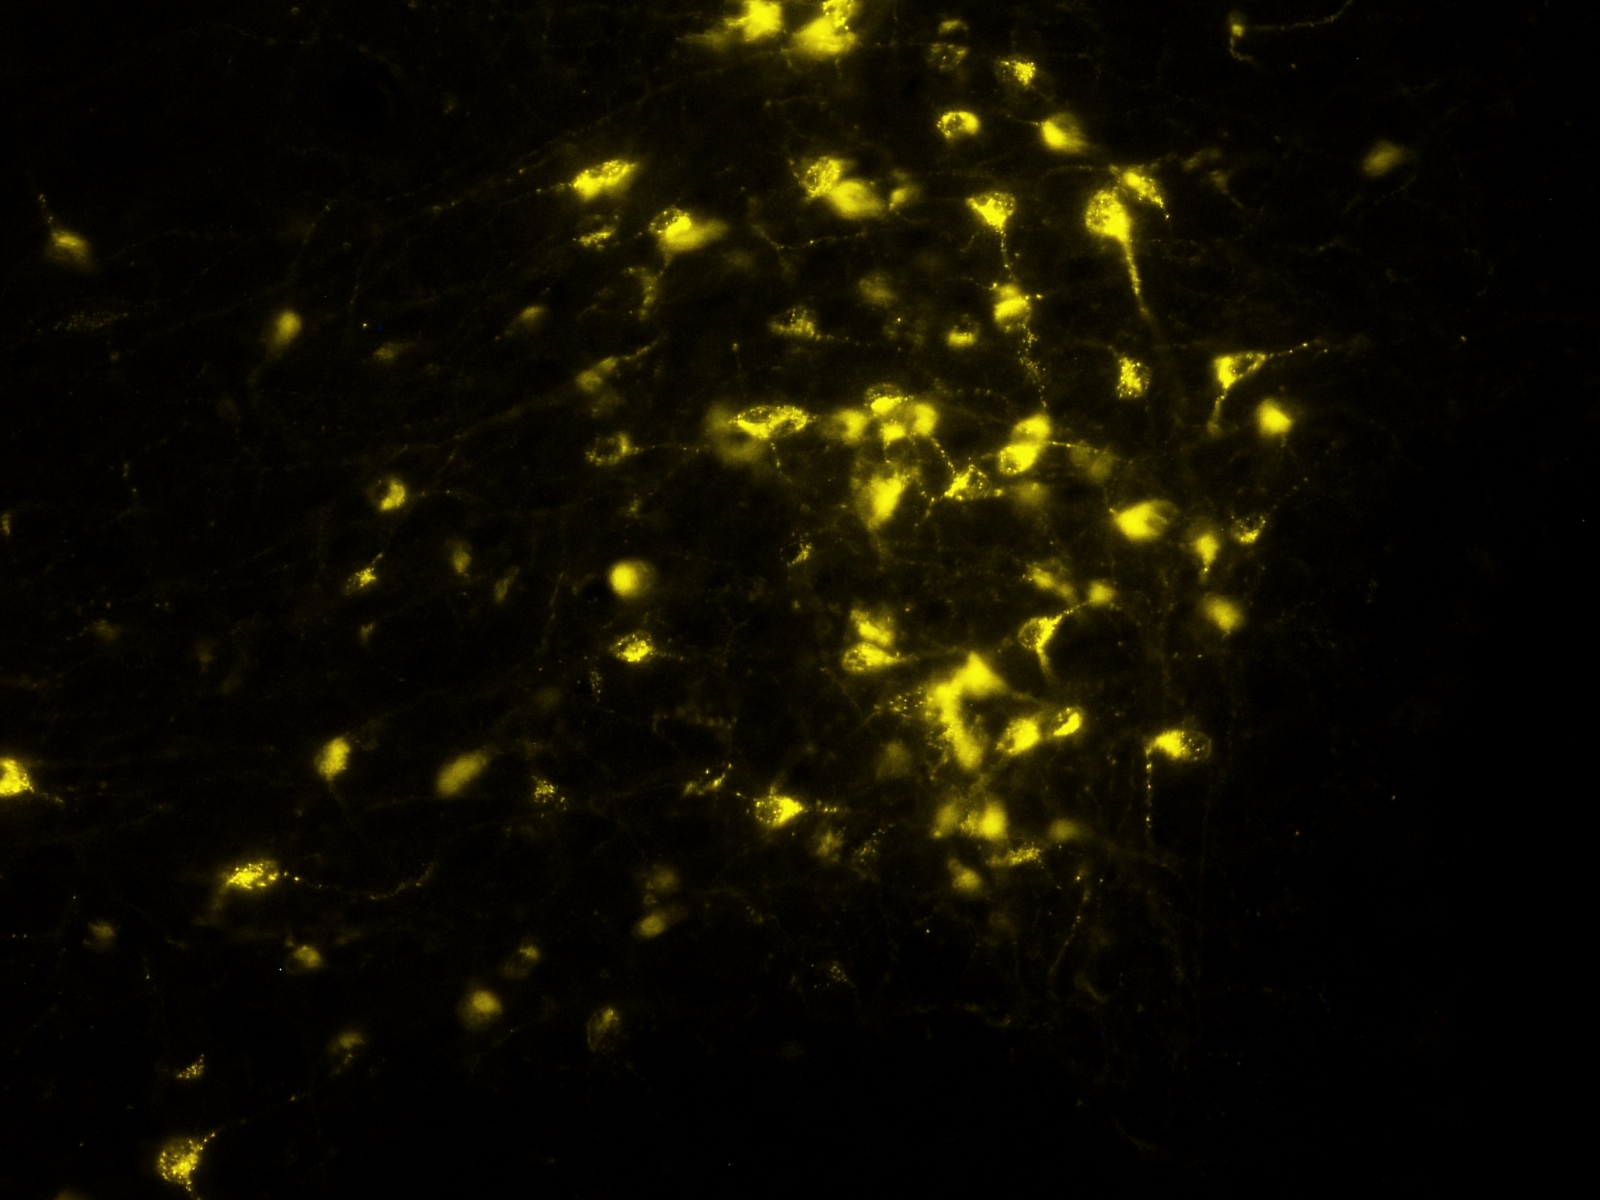
\includegraphics[width=\linewidth]{figures/120_dataset/i_clumping_yellow.png}
% \subcaption{}
% \end{subfigure}%
% \begin{subfigure}{0.5\textwidth}
% 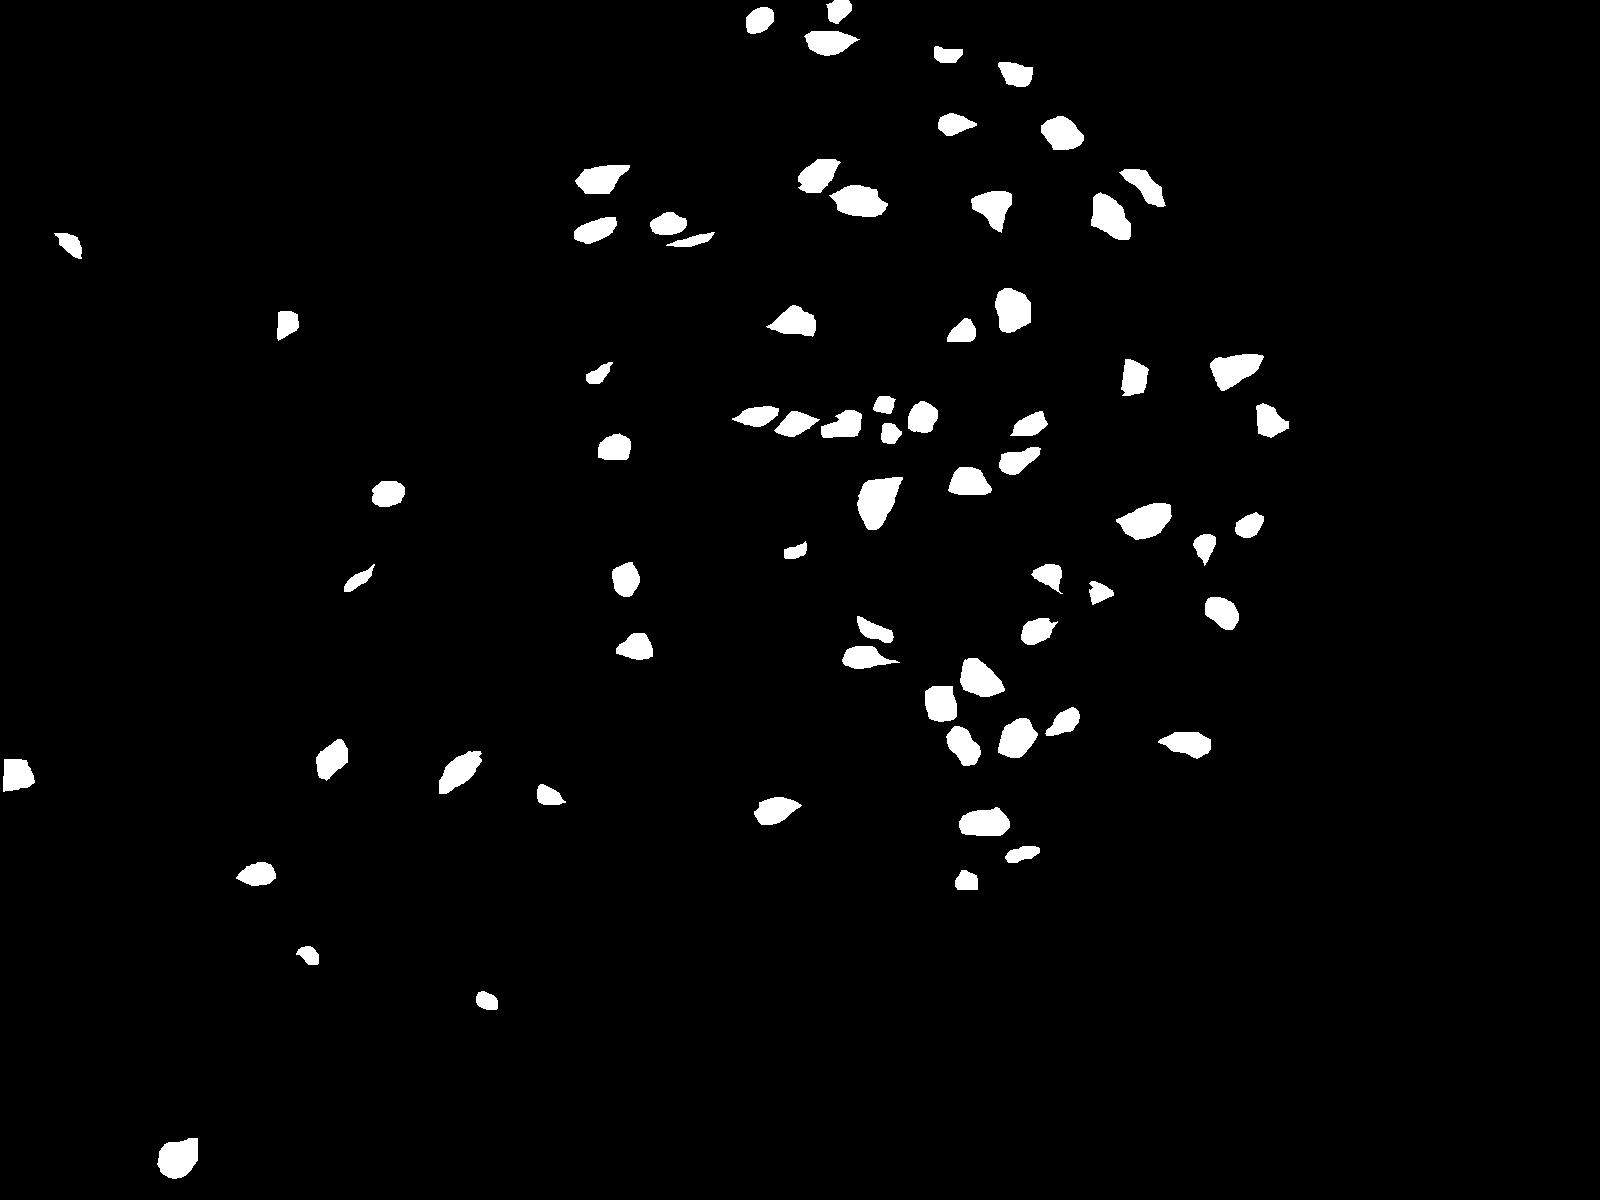
\includegraphics[width=\linewidth]{figures/120_dataset/m_clumping_yellow.png}
% \subcaption{}
% \label{fig:artifacts:clumping}
% \end{subfigure}

\begin{landscape}
\begin{figure}
    \centering
    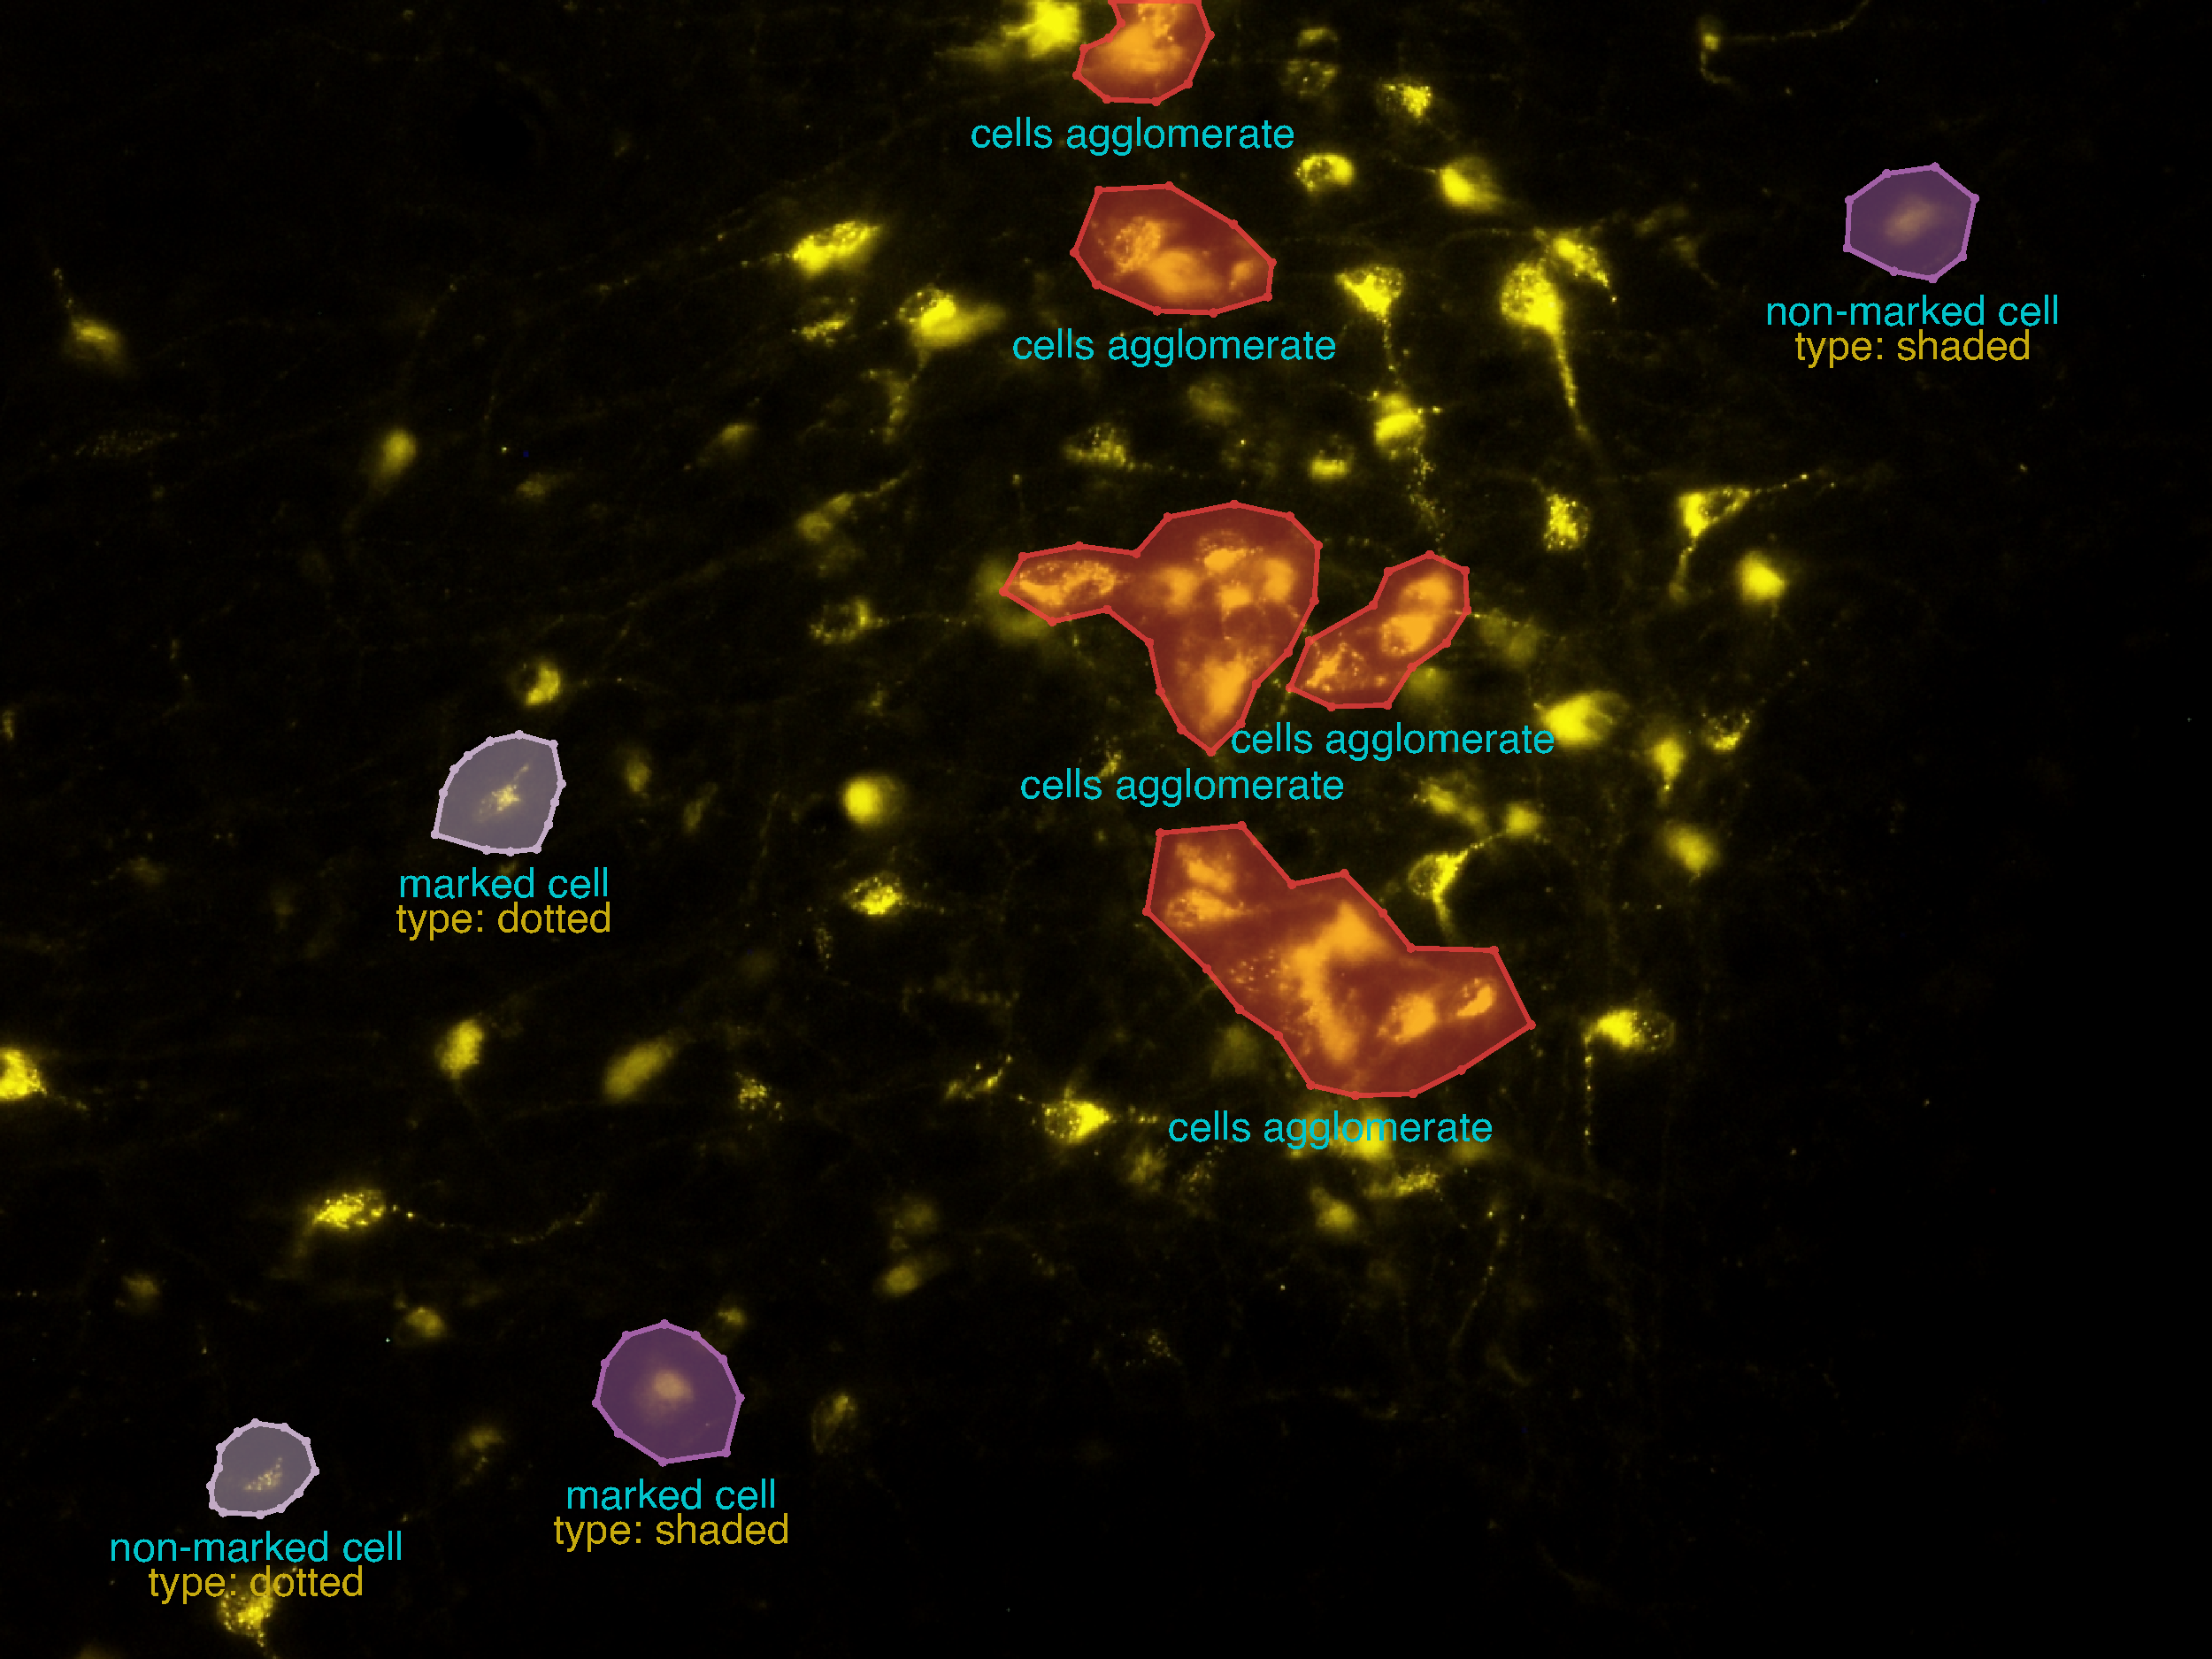
\includegraphics[width=\linewidth]{figures/120_dataset/challenges/challenges.pdf}
    \caption{Caption}
    \label{fig:artifacts:clumping}
\end{figure}
\end{landscape}

\begin{landscape}
\begin{figure}
    \centering
    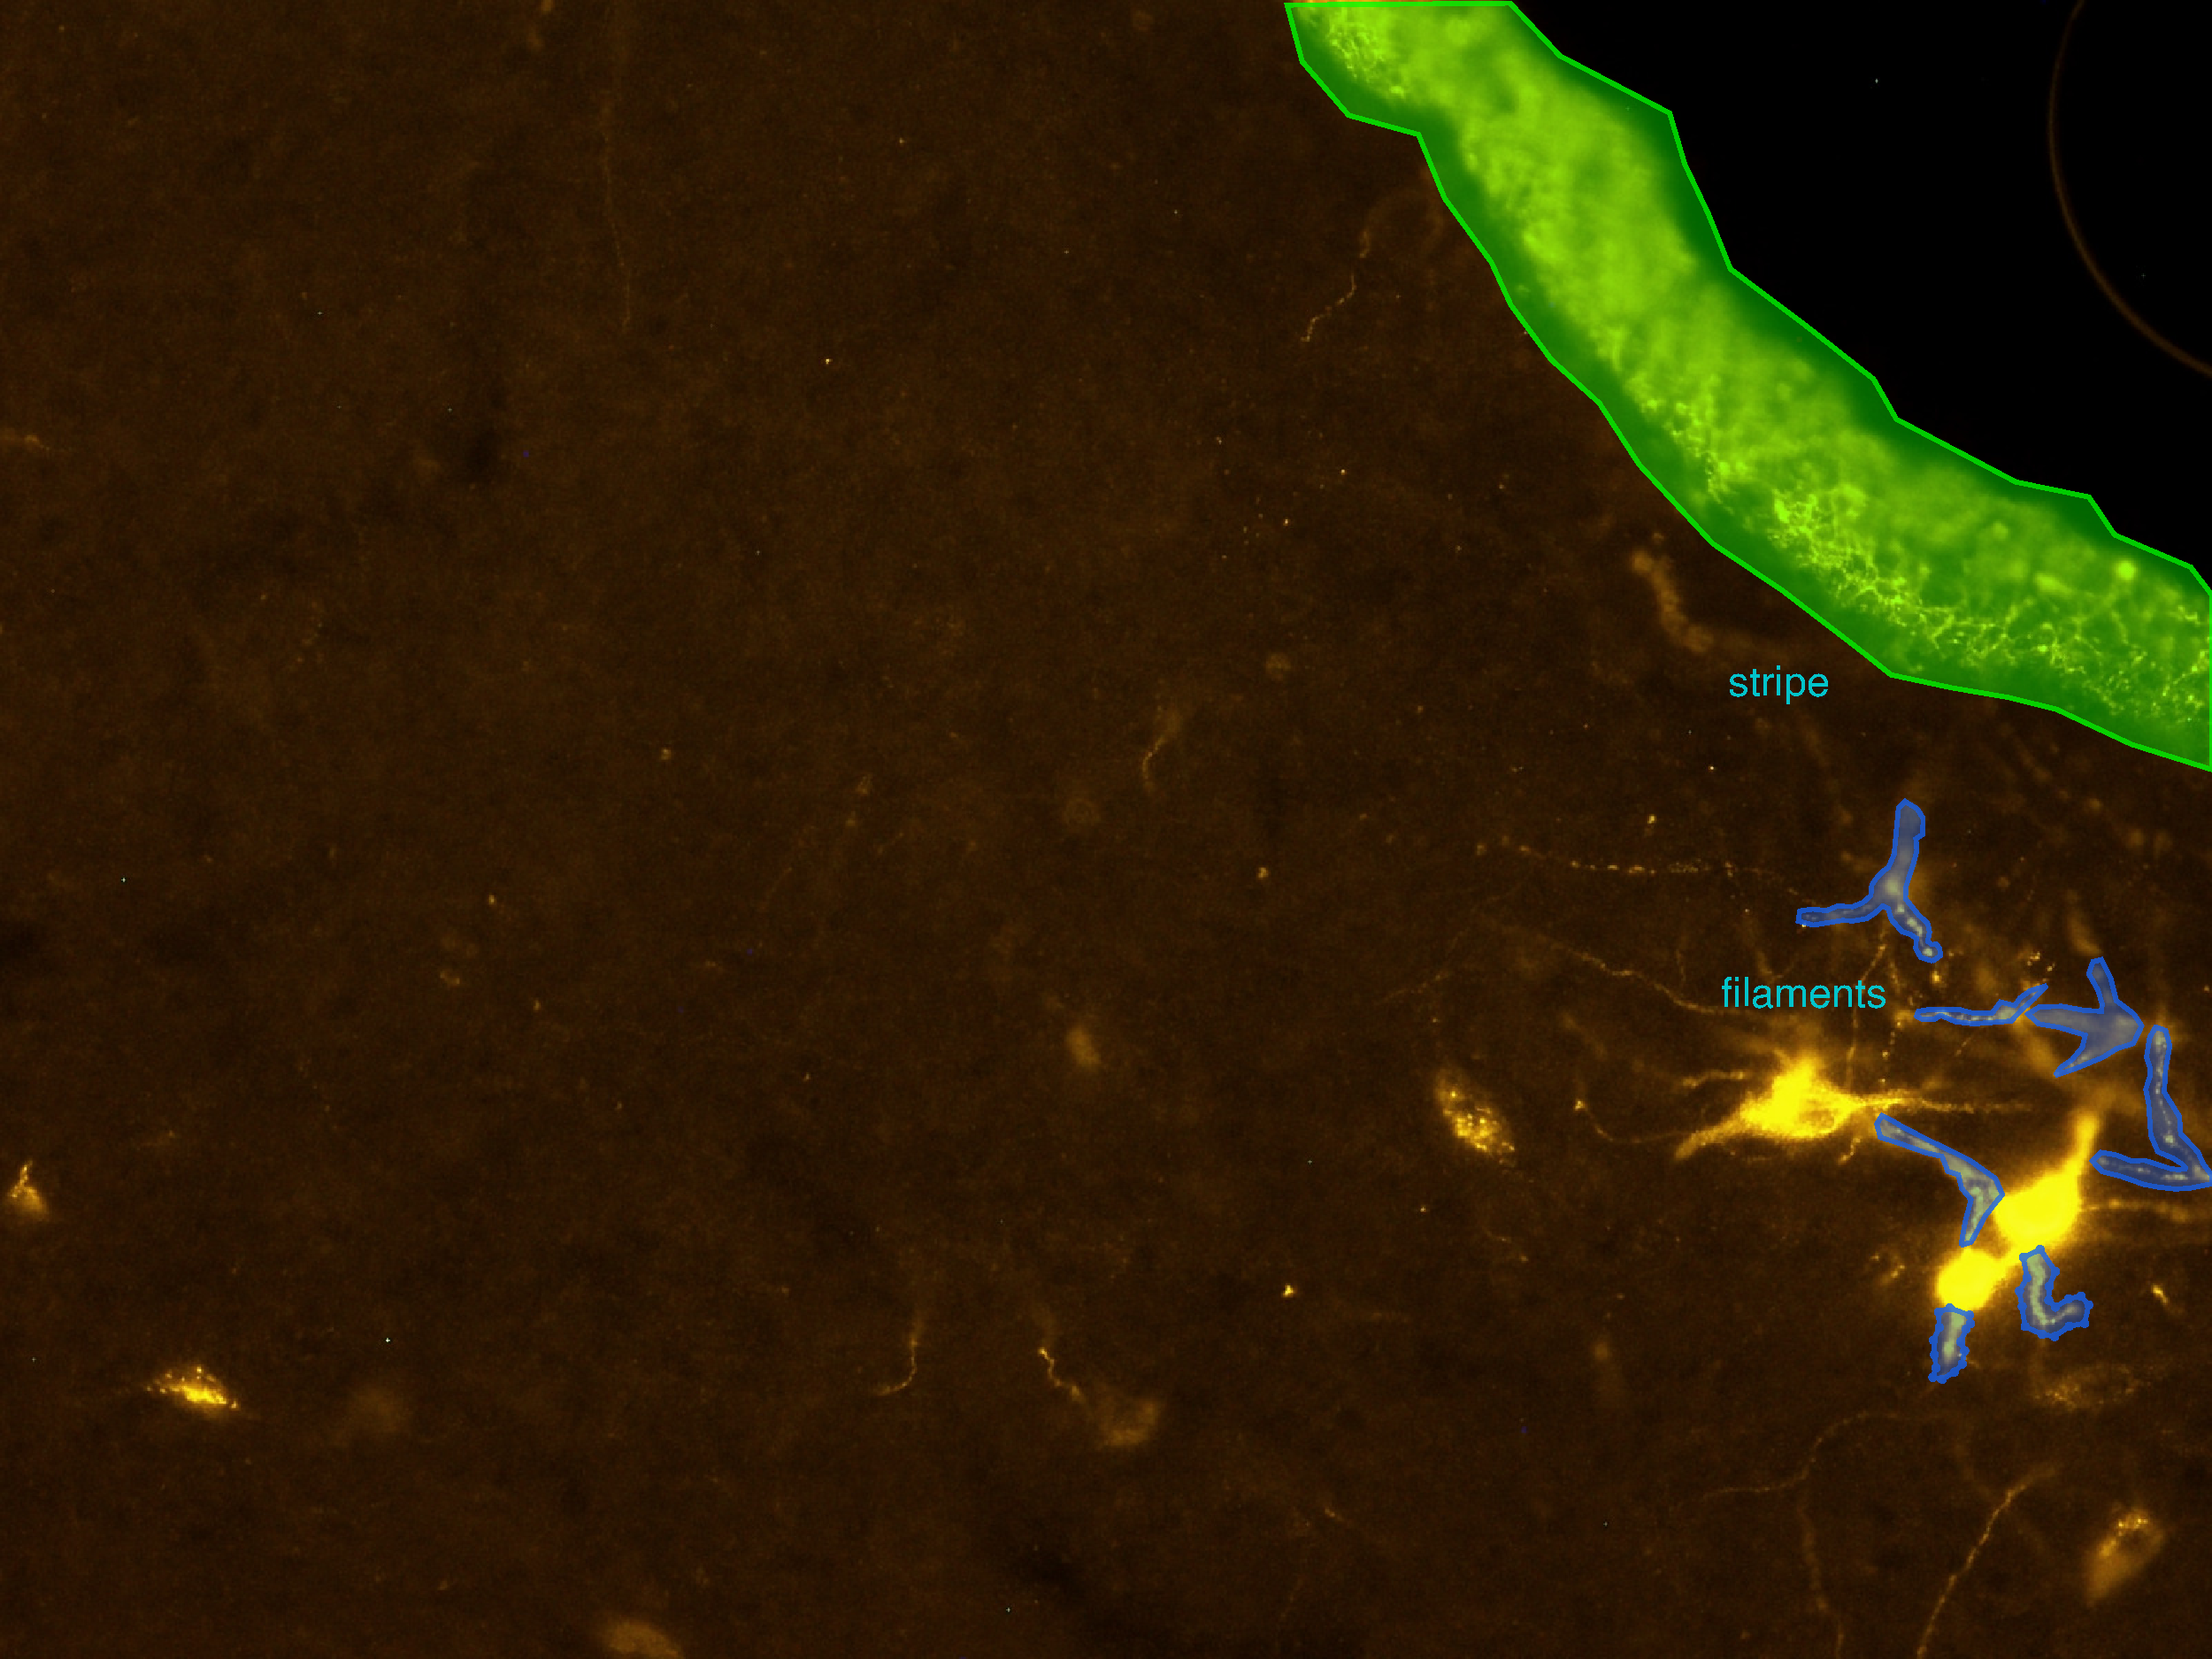
\includegraphics[width=\linewidth]{figures/120_dataset/challenges/stripe_and_filaments.pdf}
    \caption{Caption}
    \label{fig:artifacts:stripe}
\end{figure}
\end{landscape}

\begin{landscape}
\begin{figure}
    \centering
    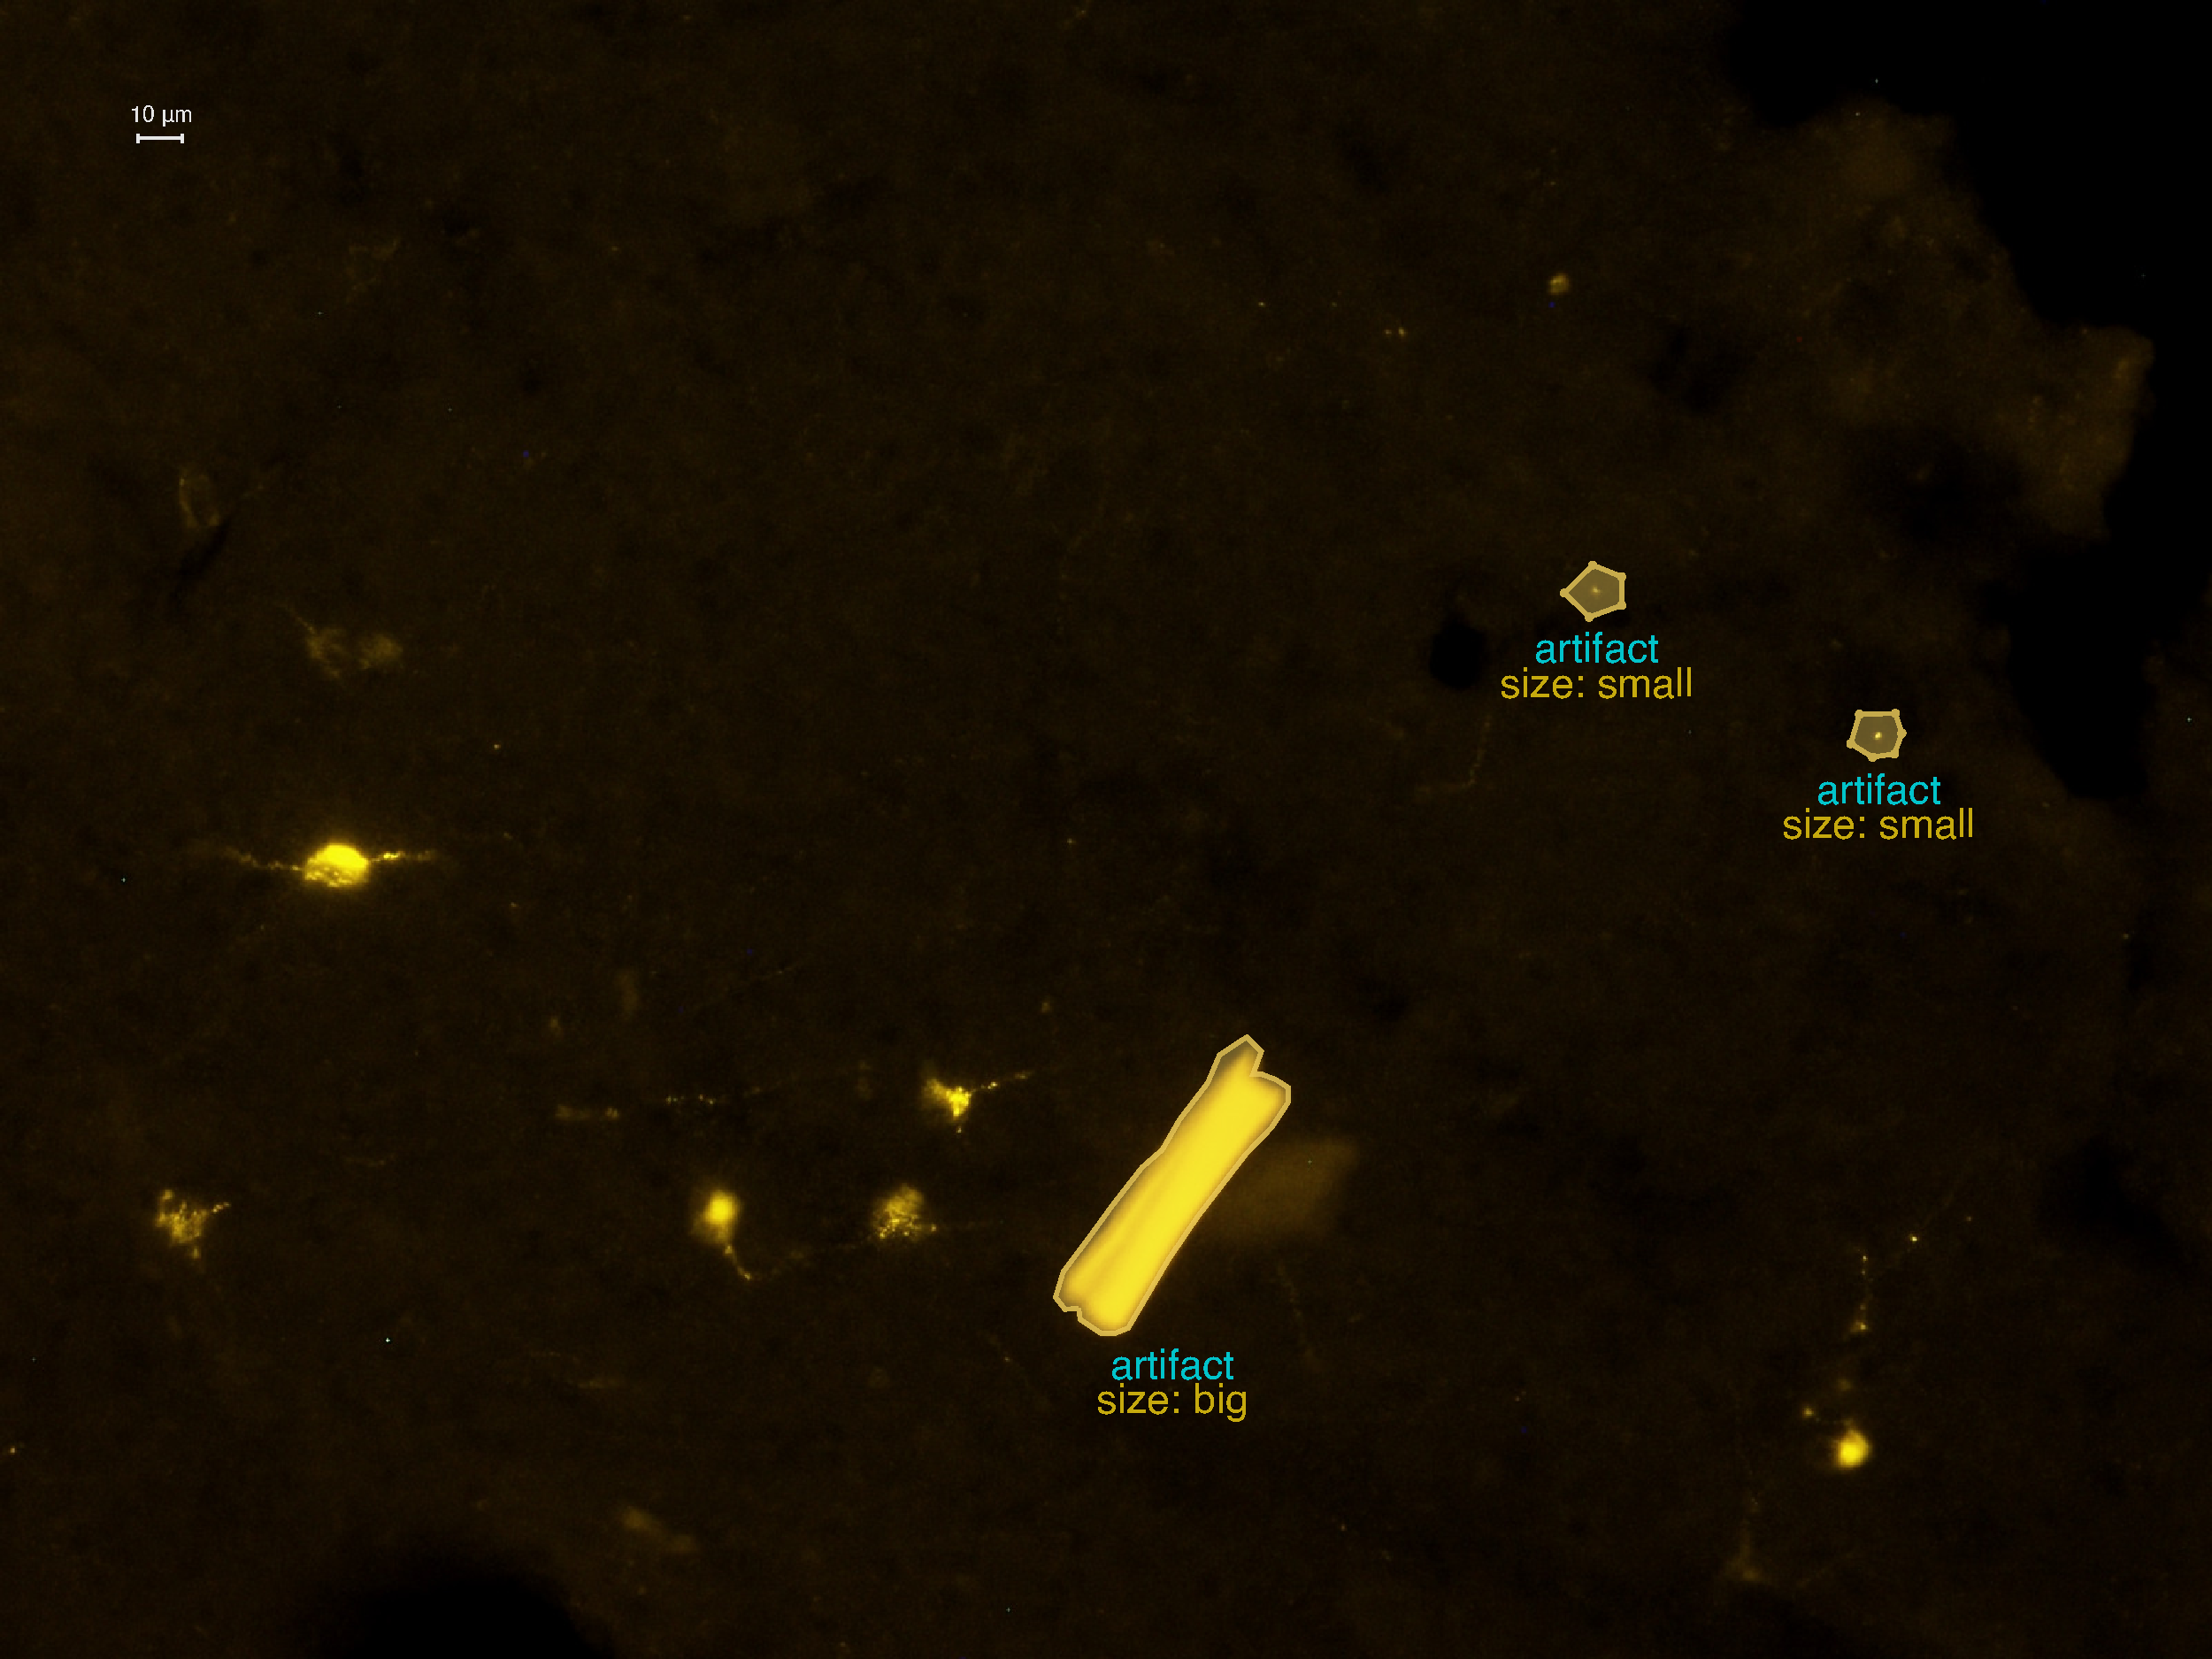
\includegraphics[width=\linewidth]{figures/120_dataset/challenges/artifacts.pdf}
    \caption{Caption}
    \label{fig:artifacts:macaroon}
\end{figure}
\end{landscape}